\documentclass{llncs}

\usepackage{fancyhdr}
\usepackage{flushend}
\usepackage{amsfonts,amssymb,amsmath,alltt}
\usepackage{stmaryrd}
\usepackage{xspace}
\usepackage{graphicx}
\usepackage{color}

\usepackage{makeidx}
\pagestyle{plain}
\usepackage[utf8]{inputenc}
\usepackage{url}
\usepackage[english]{babel}


\renewcommand{\ttdefault}{cmtt}
%This version DOES NOT suppress line breaks
% newcommands etc
\newenvironment{ttbox}{\begin{alltt}\ttbraces\small\tt}%
                      {\end{alltt}}
%the new definition of \. suppresses line breaks
\def\ttbraces{\let\.=\nobreak\chardef\{=`\{\chardef\}=`\}\chardef\|=`\\}

\newcommand{\symb}[1]{\makebox{\it #1}} 
\newcommand\ie{i.e.\!\,, }
\newcommand\rel{Re${\cal{L}}$}
\newcommand{\TODO}[1]{\textcolor{red}{\textbf{[TODO:#1]}}}
\newcommand\ttand{\mbox{{$\land$}}}
\newcommand\ttor{\mbox{{$\lor$}}}
\newcommand\ttcap{\mbox{{$\cap$}}}
\newcommand\ttcup{\mbox{{$\cup$}}}
\newcommand\ttfun{\mbox{{$\Rightarrow$}}}
\newcommand\ttmimp{\mbox{{$\Longrightarrow$}}}
\newcommand\ttimp{\mbox{{$\longrightarrow$}}}
\newcommand\ttequiv{\mbox{{$\equiv$}}}
\newcommand\ttexists{\mbox{{$\exists$}}}
\newcommand\ttforall{\mbox{{$\forall$}}}
\newcommand\ttneg{\mbox{{$\neg$}}}
\newcommand\ttneq{\mbox{{$\neq$}}}
\newcommand\ttin{\mbox{{$\in$}}}
\newcommand\ttnin{\mbox{{$\notin$}}}
\newcommand\ttImp{\mbox{{$\Longrightarrow$}}}
\newcommand\ttlam{\mbox{\( \lambda \)}}
\newcommand\tttimes{\mbox{\( \times \)}}
\newcommand\ttlbrack{\mbox{\(\llbracket\)}}
\newcommand\ttrbrack{\mbox{\( \rrbracket \)}}
\newcommand\noie{\textit{i.e.},\xspace}
\newcommand\eg{~\textit{e.g.},\xspace}
\newcommand\noeg{\textit{e.g.},\xspace}
\newcommand\ttatI{\mbox{\( @_G \)}}
\newcommand\ttto[1]{\mbox{{$\to^{#1}$}}}
\newcommand\ttleq{\mbox{{$\le$}}}
\newcommand\ttrelI{\mbox{{$\to_{i}$}}}
\newcommand\ttalpha{\mbox{{$\alpha$}}}
\newcommand\tttau{\mbox{{$\tau$}}}
\newcommand\ttsubseteq{\mbox{{$\subseteq$}}}
\newcommand\ttf{\mbox{{$f$}}}
\newcommand\ttvdash{\mbox{{$\vdash$}}}
\newcommand\ttref[1]{\mbox{\(\sqsubseteq_{#1}\)}}
\newcommand\ttNatt{\mbox{{$\mathcal{N}$}}}
\newcommand\ttattand[1]{\mbox{{$\oplus_{\wedge}^{#1}$}}}
\newcommand\ttattor[1]{\mbox{{$\oplus_{\vee}^{#1}$}}}
\newcommand\ttrelIstar{\mbox{{$\to_{i}^*$}}}


\begin{document}
\frontmatter
  
\mainmatter
\title{Modeling and analyzing the Corona-virus warning app with the Isabelle Infrastructure framework}
\author{Florian Kamm\"uller and Bianca Lutz}

\institute{Middlesex University London and\\ Technische Universit\"at Berlin\\
\email{f.kammueller@mdx.ac.uk|bialut@gmail.com}
}
\maketitle
\begin{abstract}
We provide a model in the Isabelle Infrastructure framework of the recently published
Corona-virus warning app. The app supports breaking infection chains by informing users
whether they have been in close contact to an infected person. The app has a decentralized
architecture that supports anonymity of users.
We provide a formal model of the existing app with the Isabelle Infrastructure framework
to show up some natural attacks in a very abstract model. We then use the security
refinement process of the Isabelle Infrastructure framework to highlight how the use of
continuously changing ephemeral ids improves the anonymity.
\end{abstract}

\section{Introduction}
\label{sec:intro}
The German Chancellor Angela Merkel has strongly supported the publication of
the mobile phone Corona warning app by publicly proclaiming that the ``Corona
App deserves your trust'' \cite{bundes:20}. Many millions of mobile phone users
in Germany have downloaded the app with 6 million on the first day.
This app is one amongst many similar application that aim at the very important goal
to ``break infection chains'' by providing timely information of users whether they
have been exposed to close contact with a person that has been infected.

The Corona-virus warning app has taken a long time to develop being published only on
16th June 2020. It was a quite costly project but this was mainly due to the management of
Telekom and SAP being in the driving seat. But the app has been designed with great
attention on privacy:  a distributed architecture \cite{} has been adopted after a long and
heated debate with supporters of a central architecture. The distributed architecture is
based on a very clever distributed application design whereby users phones are sending
highly anonymized so called ``Ephemeral IDs'' at physical locations via the Bluetooth
protocol. The app saves those IDs of people in close proximity. When at a later date an
infected person reports his infection to a central server, the unique root ID is published
and in the daily check all mobile phones connecting to the central server can download
the root IDs of infected people. Since the Ephemeral IDs can be mapped to the root ID
all Ephemeral IDs that have been saved over the last 14 days allow users phones to
regularly check whether their user has been exposed to an infected person and issue
a warning to the user. The warning issued by the Corona warning app entitles to
having a Corona test done (which at the time of writing is not normally possible).

The Isabelle Infrastructure framework \cite{kam:20a} allows modeling and analyzing
architecture and scenarios including physical and logical entities, actors, and policies
within the interactive theorem prover Isabelle supported with temporal logic, Kripke
structures, and attack trees. It has been applied for example to Insider analysis in
airplanes \cite{kam:20b}, privacy in IoT healthcare \cite{kam:18b}, and recently also
to blockchain protocols \cite{kn:20}.

%{Motivation: Why bother re-engineering a formal specification for a nicely developed privacy oriented app? physical aspects (adoption rate), formal proof etc}
The technical advantage of modeling an application in the Isabelle Insider framework lies
in (a) having explicit representations of infrastructures, actors and policies in a
formal model that (b) allows additional automated verification of security properties
within the interactive theorem prover Isabelle.
Although the Corona-virus app has been produced based on a sophisticated security
concept conceived by experts in the field, to our knowledge, no formal verification
has been involved. Even if a ``post-production'' formal specification seems pointless,
it allows to reveal weak points of the architecture, show that the measures that have
been conceived are suitable to cover those weak points. Thereby, we believe
that our current work is useful to increase the trust in the Corona-virus app necessary for
its wide adoption which in turn is crucial for it to be efficient.

In this paper, we first provide some background in Section \ref{sec:background}:
we give a detailed overview of the development history and security and privacy
relevant parts of the Corona-virus warning app (Section \ref{sec:history})
and some essential facts about the Isabelle Infrastructure framework
(Section \ref{sec:isainf}).
We then present our model (Section \ref{sec:model}) and analysis of privacy and
attacks (Section \ref{sec:ana}) before drawing some conclusions (Section \ref{sec:concl}).

The formal model in the Isabelle insider framework is fully mechanized and proved in
Isabelle (sources available \cite{kam:18smc}). 

\section{Background}
\label{sec:background}

\subsection{History of Decentralized Architecture}
\label{sec:history}

\subsection{Isabelle Infrastructure framework}
\label{sec:isainf}
\TODO{Adapt: this is copied from FMBC paper}
The Isabelle Infrastructure is built in the interactive generic theorem prover
Isabelle/HOL \cite{npw:02}. As a framework, it supports formalisation and proof of
systems with actors and policies. It originally emerged from verification of insider 
threat scenarios but it soon became clear that the theoretical concepts, like temporal
logic combined with Kripke structures and a generic notion of state transitions were
very suitable to be combined with attack trees into a formal security engineering process
\cite{suc:16} and framework \cite{kam:19a}.

Figure \ref{fig:theorystruc} gives an overview of the Isabelle Infrastructure 
framework with its layers of object-logics -- each level below embeds the one
above showing the novel contribution of this paper in blue on the top. 
\begin{figure}
\begin{center}
  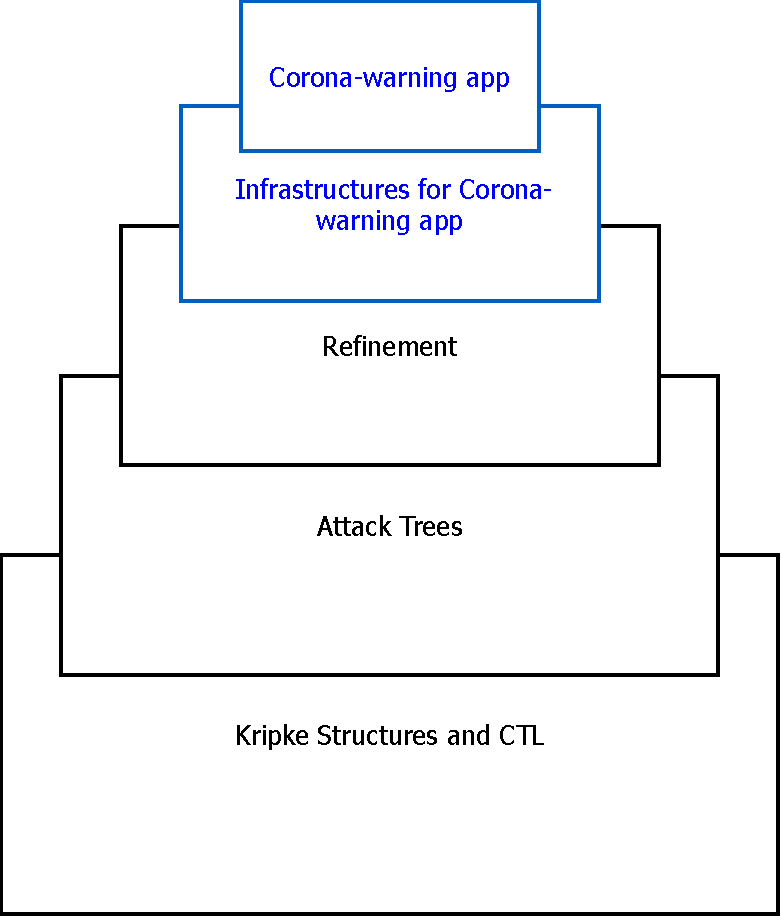
\includegraphics[scale=.5]{theory_structure.pdf}
\end{center}
%\vspace{-.5cm}
\caption{Generic Isabelle Infrastructure framework applied to Corona-warning app.}
\label{fig:theorystruc}
\end{figure}
The formal model of the Corona-warning app uses the Isabelle Infrastructure framework instantiating it
by reusing its concept of {\it actors} for users and smartphones whereby locations correspond
to physical locations. The Ephermeral IDs, their sending and change is added to Infrastructures
by slightly adapting the basic state type of infrastructure graphs and accordingly the semantic rules
for the actions move, get, and put. The details of the newly adapted Infrastructure are
presented in Section \ref{sec:model}.
Technically, an Isabelle theory file \texttt{Infrastructure.thy} builds on top of the theories for Kripke 
structures and CTL (\texttt{MC.thy}), attack trees (\texttt{AT.thy}), and security refinement 
(\texttt{Refinement.thy}). Thus all these concepts can be used to specify the formal model
for IBC, express relevant and interesting properties and conduct interactive proofs (with the 
full support of the powerful and highly automated proof support of Isabelle).
The IBC theory itself is an adaptation of the Infrastructure theory of the 
Isabelle Infrastructure framework and reuses (or slightly adapts) existing concepts. 
In the remainder of this paper, we introduce the model that we conceived for IBC. 
All Isabelle sources are available online \cite{kam:20gitsc}.


\section{Model}
\label{sec:model}

\section{Analysis}
\label{sec:ana}

\section{Conclusions}
\label{sec:concl}

\bibliographystyle{abbrv}
\bibliography{insider}

\end{document}
